% Options for packages loaded elsewhere
\PassOptionsToPackage{unicode}{hyperref}
\PassOptionsToPackage{hyphens}{url}
%
\documentclass[
  12pt,
]{article}
\usepackage{amsmath,amssymb}
\usepackage{iftex}
\ifPDFTeX
  \usepackage[T1]{fontenc}
  \usepackage[utf8]{inputenc}
  \usepackage{textcomp} % provide euro and other symbols
\else % if luatex or xetex
  \usepackage{unicode-math} % this also loads fontspec
  \defaultfontfeatures{Scale=MatchLowercase}
  \defaultfontfeatures[\rmfamily]{Ligatures=TeX,Scale=1}
\fi
\usepackage{lmodern}
\ifPDFTeX\else
  % xetex/luatex font selection
\fi
% Use upquote if available, for straight quotes in verbatim environments
\IfFileExists{upquote.sty}{\usepackage{upquote}}{}
\IfFileExists{microtype.sty}{% use microtype if available
  \usepackage[]{microtype}
  \UseMicrotypeSet[protrusion]{basicmath} % disable protrusion for tt fonts
}{}
\makeatletter
\@ifundefined{KOMAClassName}{% if non-KOMA class
  \IfFileExists{parskip.sty}{%
    \usepackage{parskip}
  }{% else
    \setlength{\parindent}{0pt}
    \setlength{\parskip}{6pt plus 2pt minus 1pt}}
}{% if KOMA class
  \KOMAoptions{parskip=half}}
\makeatother
\usepackage{xcolor}
\usepackage[margin=1in]{geometry}
\usepackage{longtable,booktabs,array}
\usepackage{calc} % for calculating minipage widths
% Correct order of tables after \paragraph or \subparagraph
\usepackage{etoolbox}
\makeatletter
\patchcmd\longtable{\par}{\if@noskipsec\mbox{}\fi\par}{}{}
\makeatother
% Allow footnotes in longtable head/foot
\IfFileExists{footnotehyper.sty}{\usepackage{footnotehyper}}{\usepackage{footnote}}
\makesavenoteenv{longtable}
\usepackage{graphicx}
\makeatletter
\def\maxwidth{\ifdim\Gin@nat@width>\linewidth\linewidth\else\Gin@nat@width\fi}
\def\maxheight{\ifdim\Gin@nat@height>\textheight\textheight\else\Gin@nat@height\fi}
\makeatother
% Scale images if necessary, so that they will not overflow the page
% margins by default, and it is still possible to overwrite the defaults
% using explicit options in \includegraphics[width, height, ...]{}
\setkeys{Gin}{width=\maxwidth,height=\maxheight,keepaspectratio}
% Set default figure placement to htbp
\makeatletter
\def\fps@figure{htbp}
\makeatother
\setlength{\emergencystretch}{3em} % prevent overfull lines
\providecommand{\tightlist}{%
  \setlength{\itemsep}{0pt}\setlength{\parskip}{0pt}}
\setcounter{secnumdepth}{5}
\newlength{\cslhangindent}
\setlength{\cslhangindent}{1.5em}
\newlength{\csllabelwidth}
\setlength{\csllabelwidth}{3em}
\newlength{\cslentryspacingunit} % times entry-spacing
\setlength{\cslentryspacingunit}{\parskip}
\newenvironment{CSLReferences}[2] % #1 hanging-ident, #2 entry spacing
 {% don't indent paragraphs
  \setlength{\parindent}{0pt}
  % turn on hanging indent if param 1 is 1
  \ifodd #1
  \let\oldpar\par
  \def\par{\hangindent=\cslhangindent\oldpar}
  \fi
  % set entry spacing
  \setlength{\parskip}{#2\cslentryspacingunit}
 }%
 {}
\usepackage{calc}
\newcommand{\CSLBlock}[1]{#1\hfill\break}
\newcommand{\CSLLeftMargin}[1]{\parbox[t]{\csllabelwidth}{#1}}
\newcommand{\CSLRightInline}[1]{\parbox[t]{\linewidth - \csllabelwidth}{#1}\break}
\newcommand{\CSLIndent}[1]{\hspace{\cslhangindent}#1}
\usepackage{setspace} \usepackage{lineno} \usepackage{placeins} \usepackage[nottoc,notlof,notlot]{tocbibind} \renewcommand{\contentsname}{} \renewcommand{\listfigurename}{} \renewcommand{\listtablename}{} \usepackage{sectsty} \sectionfont{\centering}
\usepackage{booktabs}
\usepackage{longtable}
\usepackage{array}
\usepackage{multirow}
\usepackage{wrapfig}
\usepackage{float}
\usepackage{colortbl}
\usepackage{pdflscape}
\usepackage{tabu}
\usepackage{threeparttable}
\usepackage{threeparttablex}
\usepackage[normalem]{ulem}
\usepackage{makecell}
\usepackage{xcolor}
\ifLuaTeX
  \usepackage{selnolig}  % disable illegal ligatures
\fi
\IfFileExists{bookmark.sty}{\usepackage{bookmark}}{\usepackage{hyperref}}
\IfFileExists{xurl.sty}{\usepackage{xurl}}{} % add URL line breaks if available
\urlstyle{same}
\hypersetup{
  hidelinks,
  pdfcreator={LaTeX via pandoc}}

\author{}
\date{\vspace{-2.5em}}

\begin{document}

\doublespacing

\begin{center}
    
\textbf{\Large Bibliometric Analysis of Mangroves in Fisheries}
    
\textsc{Sophie Wulfing$^{1*}$ and Rohani Ambo Rappe$^{1}$\\}
\vspace{3 mm}
\normalsize{\indent $^1$Department of Marine Ecology, Hasanuddin University, Indonesia\\}
$\text{*}$ Corresponding authors: Sophie Wulfing (SophieWulfing@gmail.com)
\end{center}

\newpage

\hypertarget{introduction}{%
\section{INTRODUCTION}\label{introduction}}

Mangroves are inter-tidal forests that are essential components to many tropical ecosystems. As the effects of climate change grow stronger worldwide, the need for carbon mitigation and protection against extreme weather are becoming more urgent. Mangroves biomes comprise about 14 \% of marine carbon sequestration and may result in high gas emissions when these ecosystems are disturbed (Alongi, 2012), while more established mangroves are more efficient in absorbing atmospheric carbon (Cameron et al., 2019). Beyond their benefits of protecting against extreme weather events, mangroves are also key actors in maintaining the biodiversity of the ecosystems they inhabit. Mangroves have been reported to support up 20\% of the benthic biodiversity in their habitats (Carugati et al., 2018). They provide essential nutrients, temperature controls, and protection from predators for marine life (Blue Forests, 2012). Further, Mangroves have been shown to increase fishery yields in their surrounding areas, therefore increasing fisher income (Aburto-Oropeza et al., 2008). The root systems of mangroves provide shelter and protection for juvenile fish, allowing them to grow and develop safely away from predators and also also act as a buffer against strong currents and waves, creating calmer and more stable environments where fish can feed and reproduce (Alongi, 2008). Areas with intact mangrove forests have been shown to support higher fish abundance and diversity compared to areas without mangroves (Nagelkerken et al., 2008). Mangroves provide a rich food web, with leaf litter and detritus serving as a source of nutrients that fuel the basis of the food chain, supporting the growth and survival of various fish species (Alongi, 2008). Furthermore, mangroves act as a buffer against coastal erosion and storm surges, safeguarding the habitats of both fish and fishermen (Nagelkerken et al., 2008). Mangroves offer a crucial line of defense against the impacts of climate change on fisheries. The dense root systems of mangroves stabilize shorelines and protect coastal areas from erosion caused by rising sea levels and extreme weather events (Alongi, 2008).

Despite all of their contributions to ecosystem health, mangrove environments are being threatened worldwide. Rising sea-levels has been shown to be a major contributor to mangrove loss (Gilman et al., 2008). Further, as extreme events are becoming more intense and more frequent, these could potentially threaten mangroves due to defoliation, soil erosion, or by altering the chemical makeup or temperature of soils (Gilman et al., 2008). Mangroves are also directly threatened by anthropogenic activity. Pollution, coastal development, and aquaculture development have also contributed to mangrove ecosystem loss (Adeel \& Pomeroy, 2002). Mangrove forests in the Western Tropical Pacific are the most diverse of these habitats globally (Ellison et al., 1999).

DISCUSSITON OF SSF AND CONNECTION TO MANGROVES AND THEN GO INTO WHY YOU'RE WRITING THIS

Bibliometric analysis is a statistical analysis of trends in research related to a specific topic.

\hypertarget{methods}{%
\section{METHODS}\label{methods}}

\hypertarget{results-and-discussion}{%
\section{RESULTS AND DISCUSSION}\label{results-and-discussion}}

When searching research articles that cover mangroves, fisheries, and biomass or biodiversity in the SCOPUS database, a total of NUMBEROFDOCS were found from a 138 different sources. Dates of publication ranged form 1989 to 2024, and 37.45\% of these articles were written with international co-Authorship. Figure \ref{AnnualScientificProduction} shows the total number of articles published which use the keywords of mangroves, fisheries and biomass or biodiversity. The greatest increase of number of papers written that covers these three topics was in 2015, when the number of articles was 7 to 2016, where the number of articles doubled to 14. The highest number of articles in this analysis was seen in 2022 with 29 articles. The journal that has published the most papers in these areas was Ocean and Coastal Management with 13 total publications. However, this journal's first paper relevant to mangroves, fisheries, and biomass or biodiversity was first published in 2005, whereas Estuarine, Coastal, and Shelf Science, the second most active journal, published it's first paper on the subject in 1989 \ref{SourceDynamics}.

and Seas at the Millennium. SOME INFORMATION ABOUT EACH JOURNAL.

However, Seas at the Millennium was \#3 a WHY DID THIS JUST HAVE ONE UPTIC.

BIODIVERSITAS COMES IN 4TH BEHIND MARINE POLLUTION BULLETIN. iS THIS THE FIRST NON-ENGLISH LANGUAGE JOURNAL?

In terms of geographic distribution of research on mangroves, fisheries, and biomass or biodiversity, Australia has the highest number of total authorship as well as the highest number of secondary authorship whereas the country with the most Main Corresponding authors is the United States. The United States also has the highest number of cited documents, with 3,625 total citations (Figure \ref{AuthorCountries}). MAKE MAP OUT OF COUNTRY\_PRODUCTION DOCUMENT WITH COUNTRY TITLES.

Keyword trends are helpful indicators of WHAT IS RELEVANT IN SCIENCE IDK LOL. Figure \ref{TrendTopics}shows the most relevant keywords (used more than ten times total and over three times a year) and which years they have been the most used. Most recently, the terms carbon, human, and climate change have become the most relevant topics. This is likely due to SAY SOME MANGROVE FAKTS LIKE THEIR DESTRUCTION UNDER HUMNA INFLUENCE AND THEIR HELP AGAINST CLIMATE CHANGE. MAYBE SOMETHING ABOUT THE INDIAN OCEAN, IDK

\hypertarget{collaborations}{%
\subsection{Collaborations}\label{collaborations}}

Figure \ref{CountryCollaborationNetwork} shows the amount of authorship collaboration that occurs between each country. By far, the greatest amount of authorship collaboration that occurs is between the US and Australia. SOME DISCUSSION ABOUT GEOGRAPHICAL DISTRIBUTION OF MANGROVES

\begin{figure}
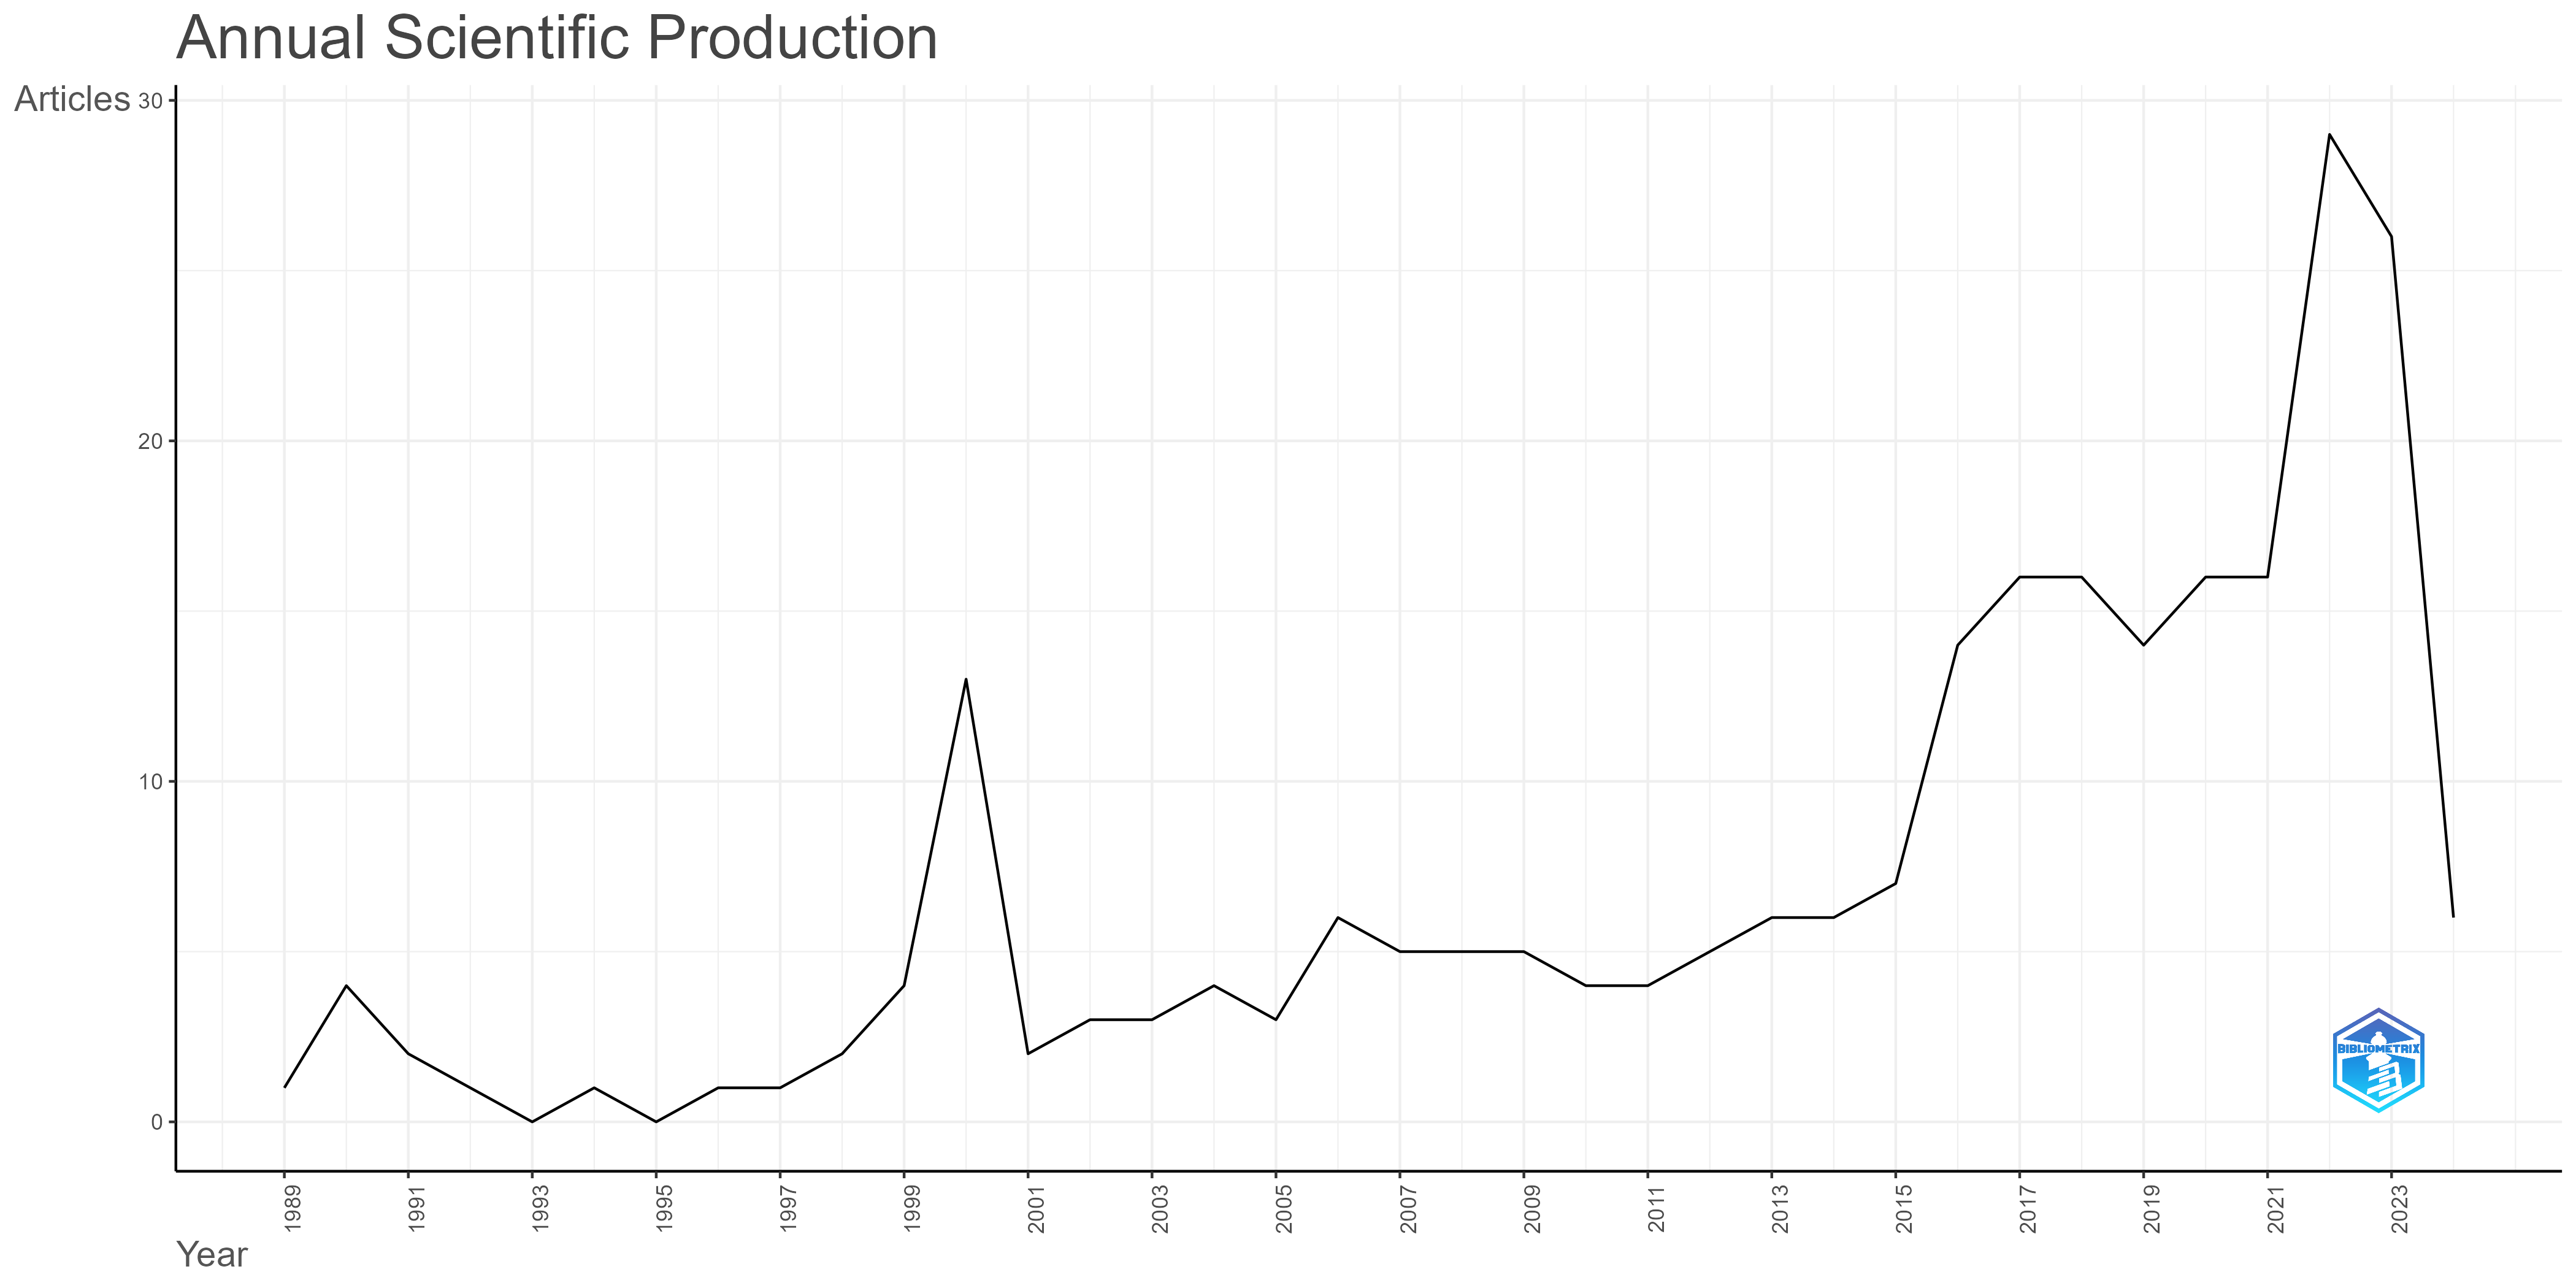
\includegraphics[width=1\linewidth]{AnnualScientificProduction} \caption{Fig Cap \label{AnnualScientificProduction}}\label{fig:AnnualScientificProduction}
\end{figure}



\begin{figure}
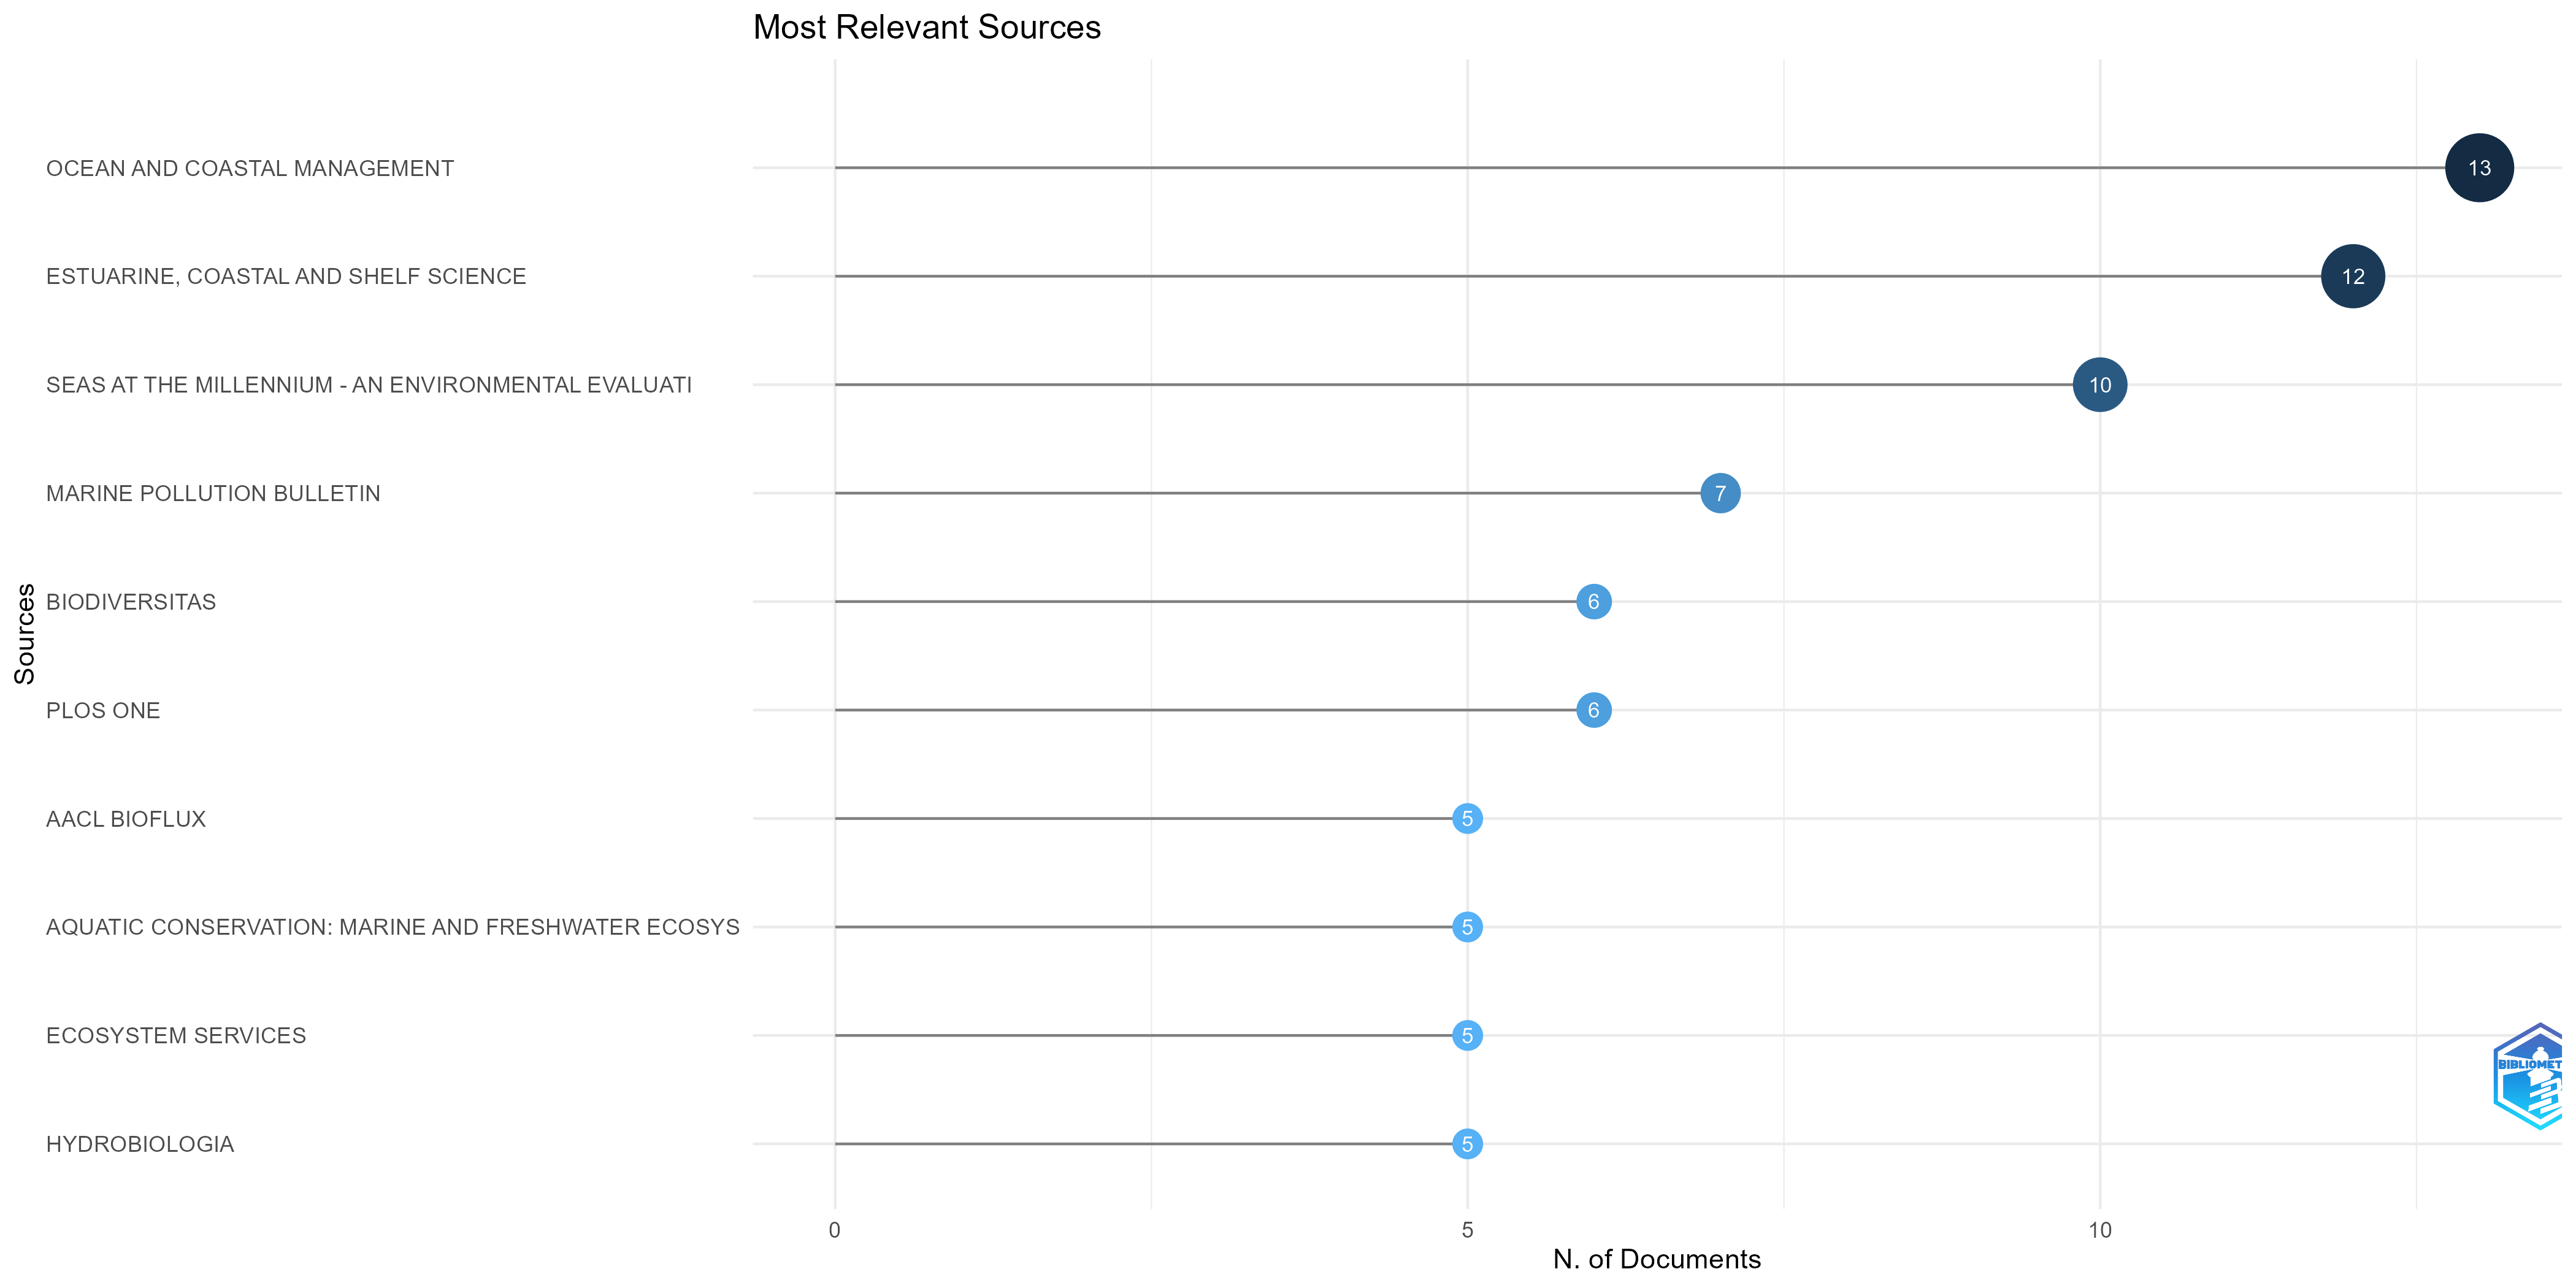
\includegraphics[width=0.5\linewidth]{MostRelevantSources} 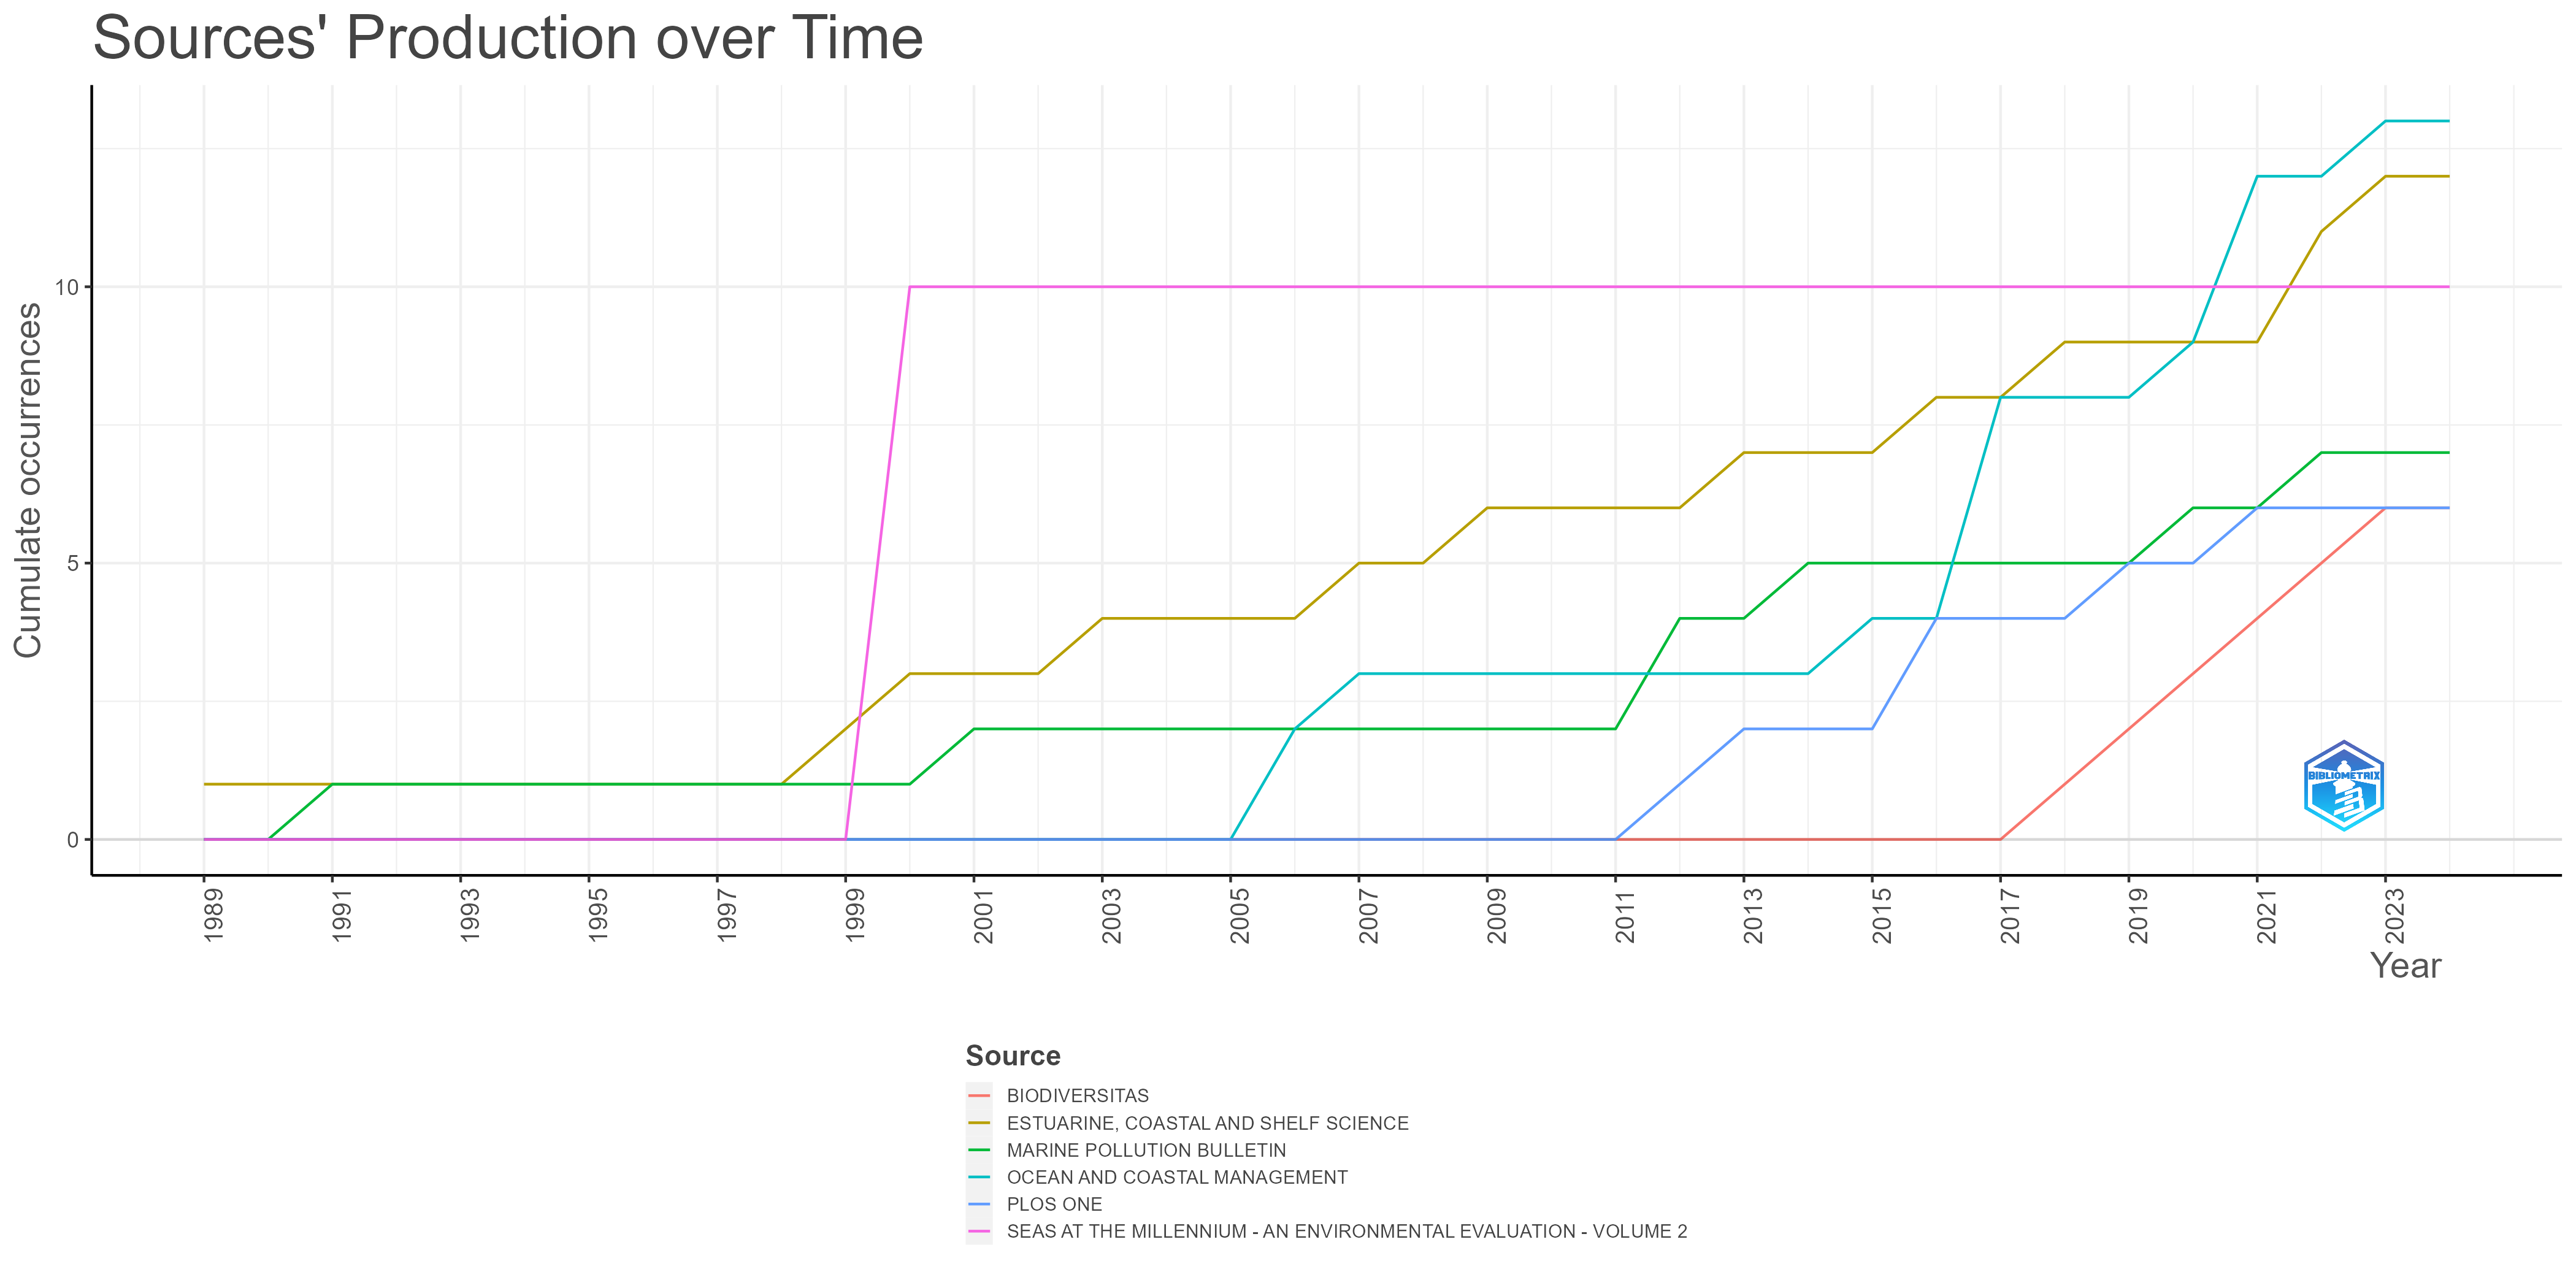
\includegraphics[width=0.5\linewidth]{SourceDynamics} \caption{Fig Cap \label{SourceDynamics}}\label{fig:SourceDynamics}
\end{figure}



\begin{figure}
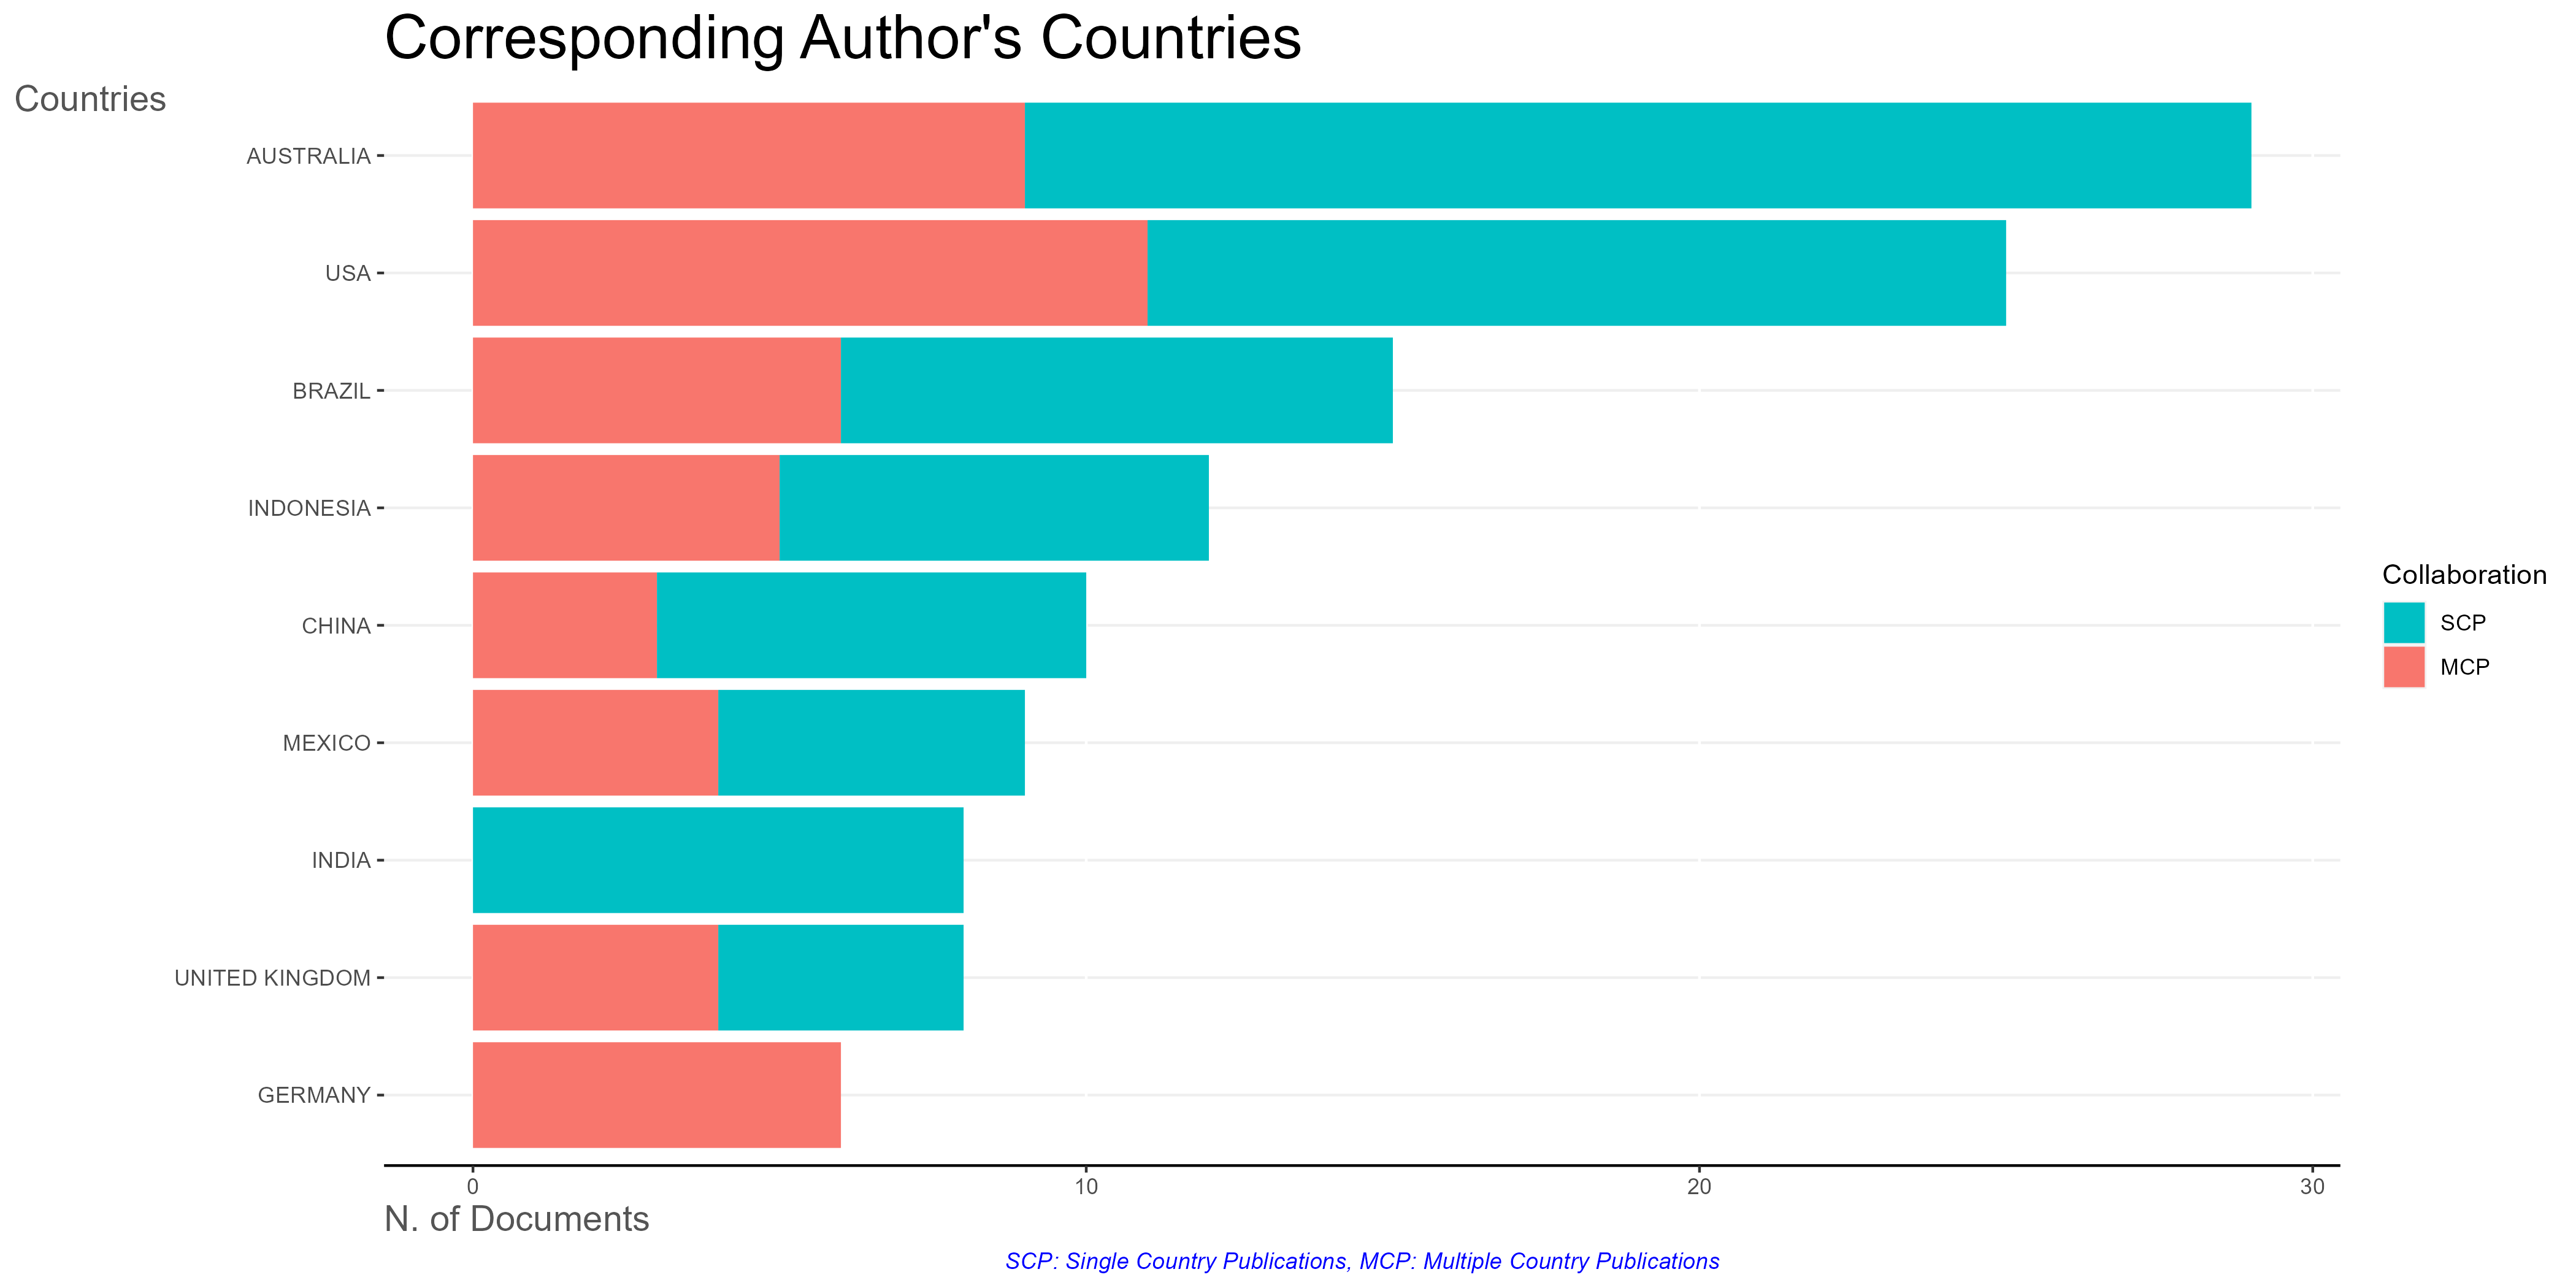
\includegraphics[width=1\linewidth]{AuthorCountries} \caption{Fig Cap \label{AuthorCountries}}\label{fig:AuthorCountries}
\end{figure}



\begin{figure}
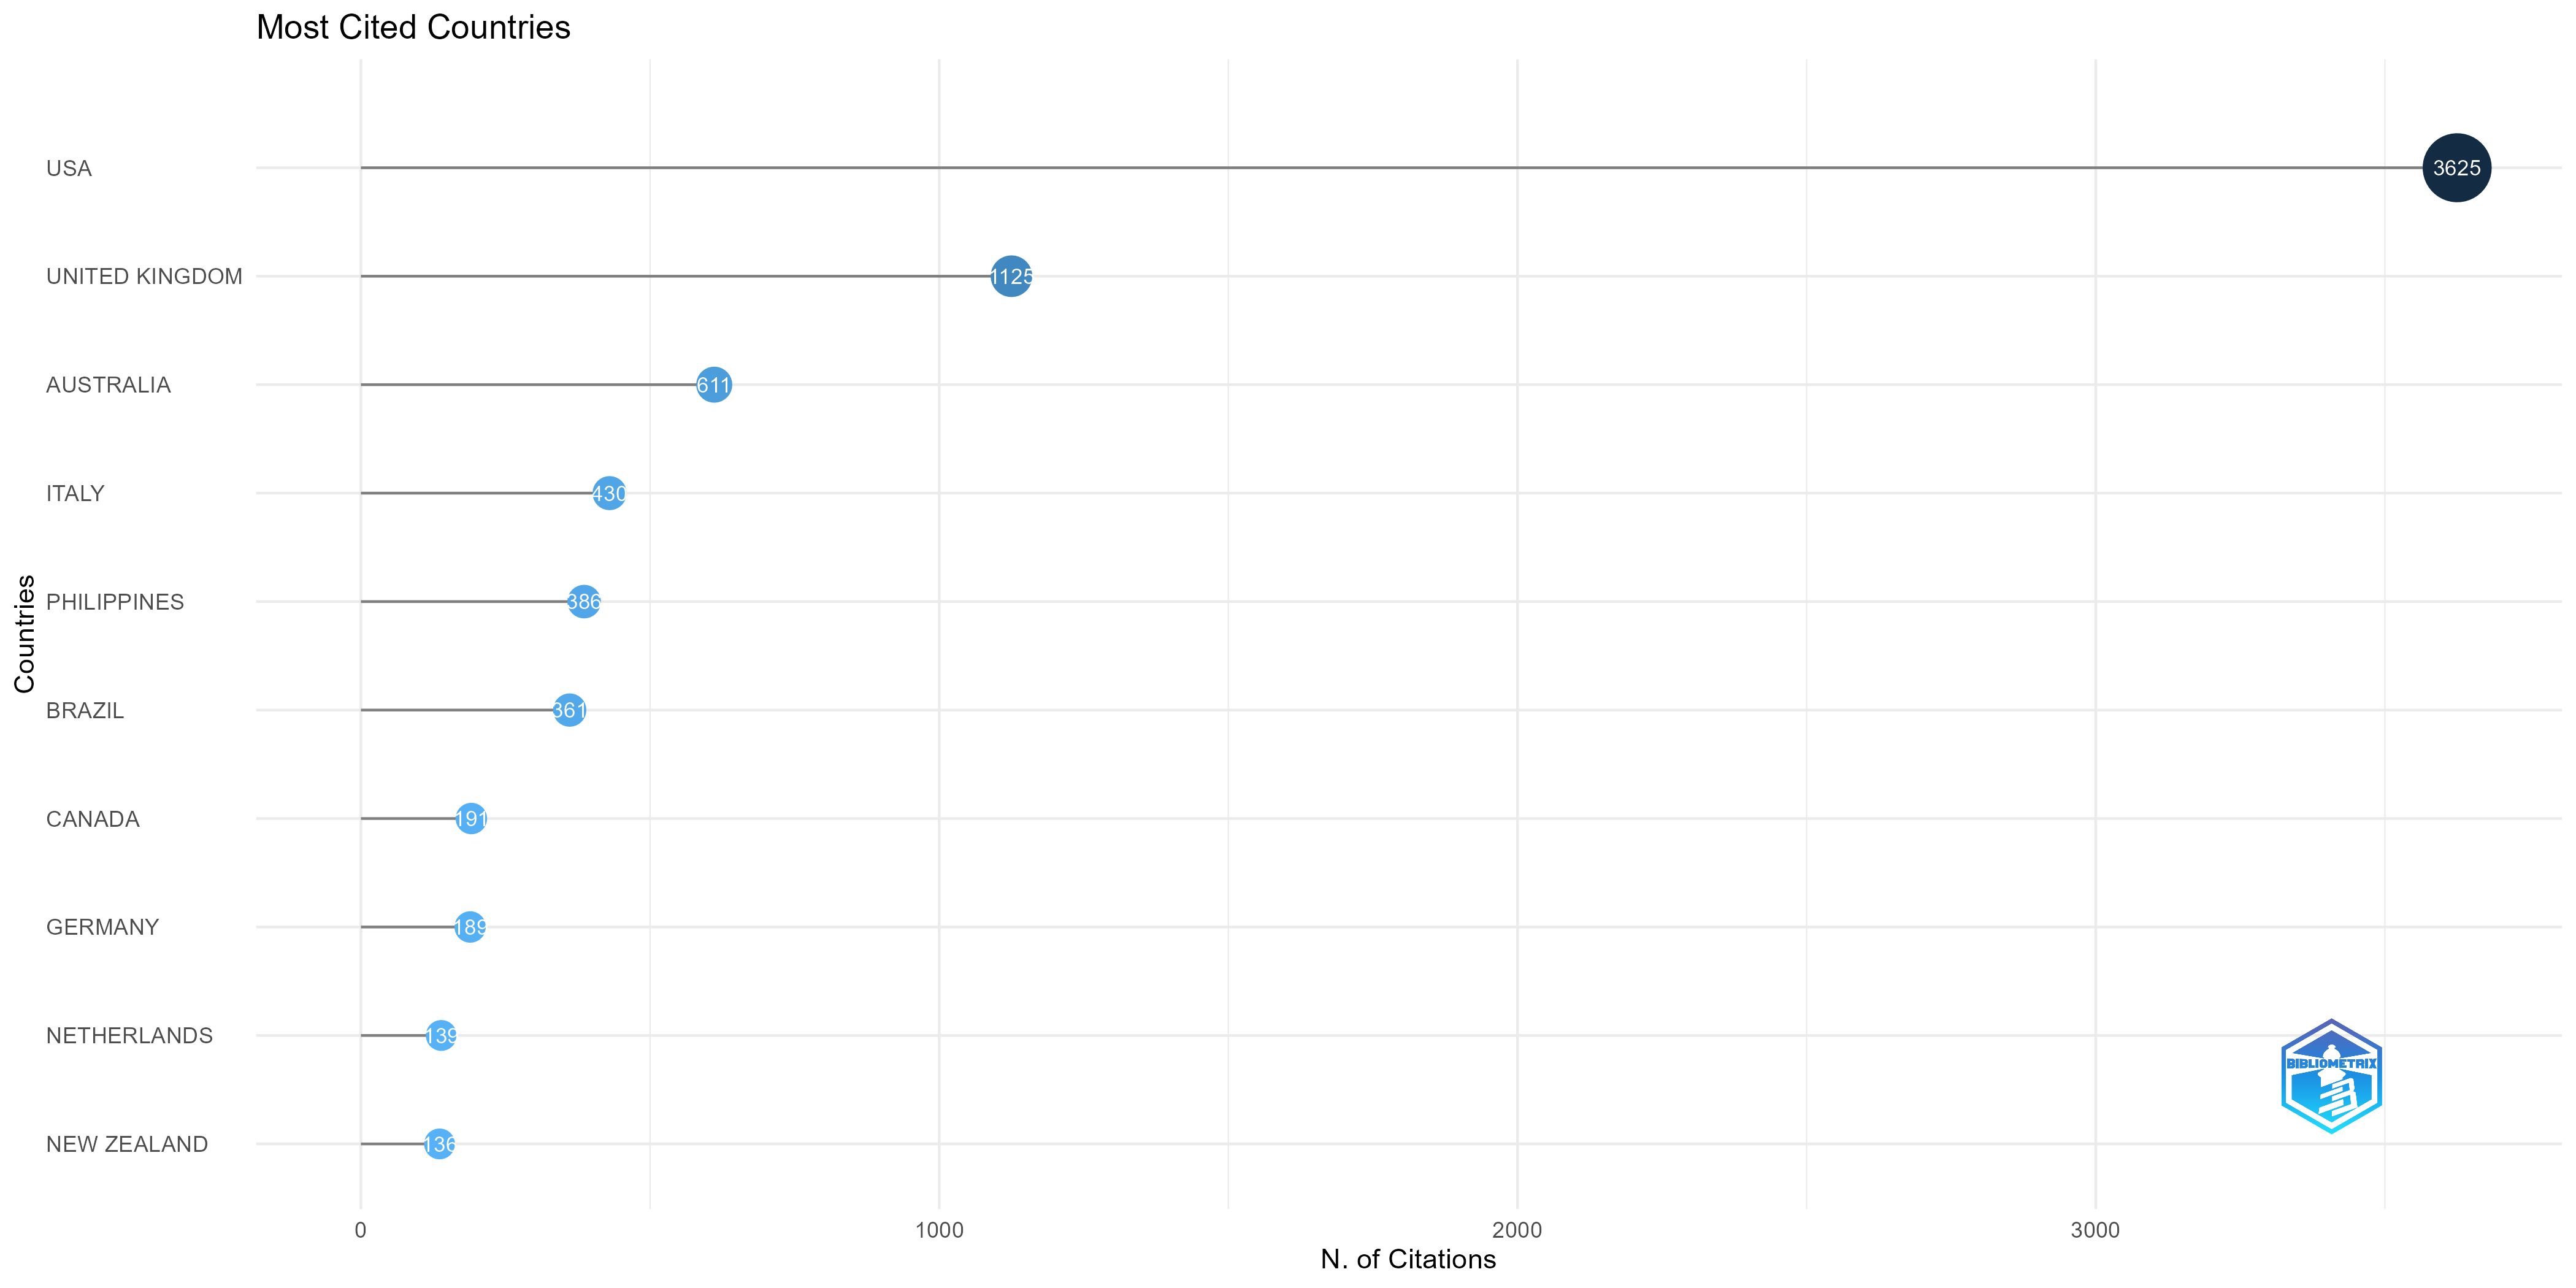
\includegraphics[width=1\linewidth]{MostCitedCountries} \caption{Fig Cap \label{MostCitedCountries}}\label{fig:MostCitedCountries}
\end{figure}



\begin{figure}
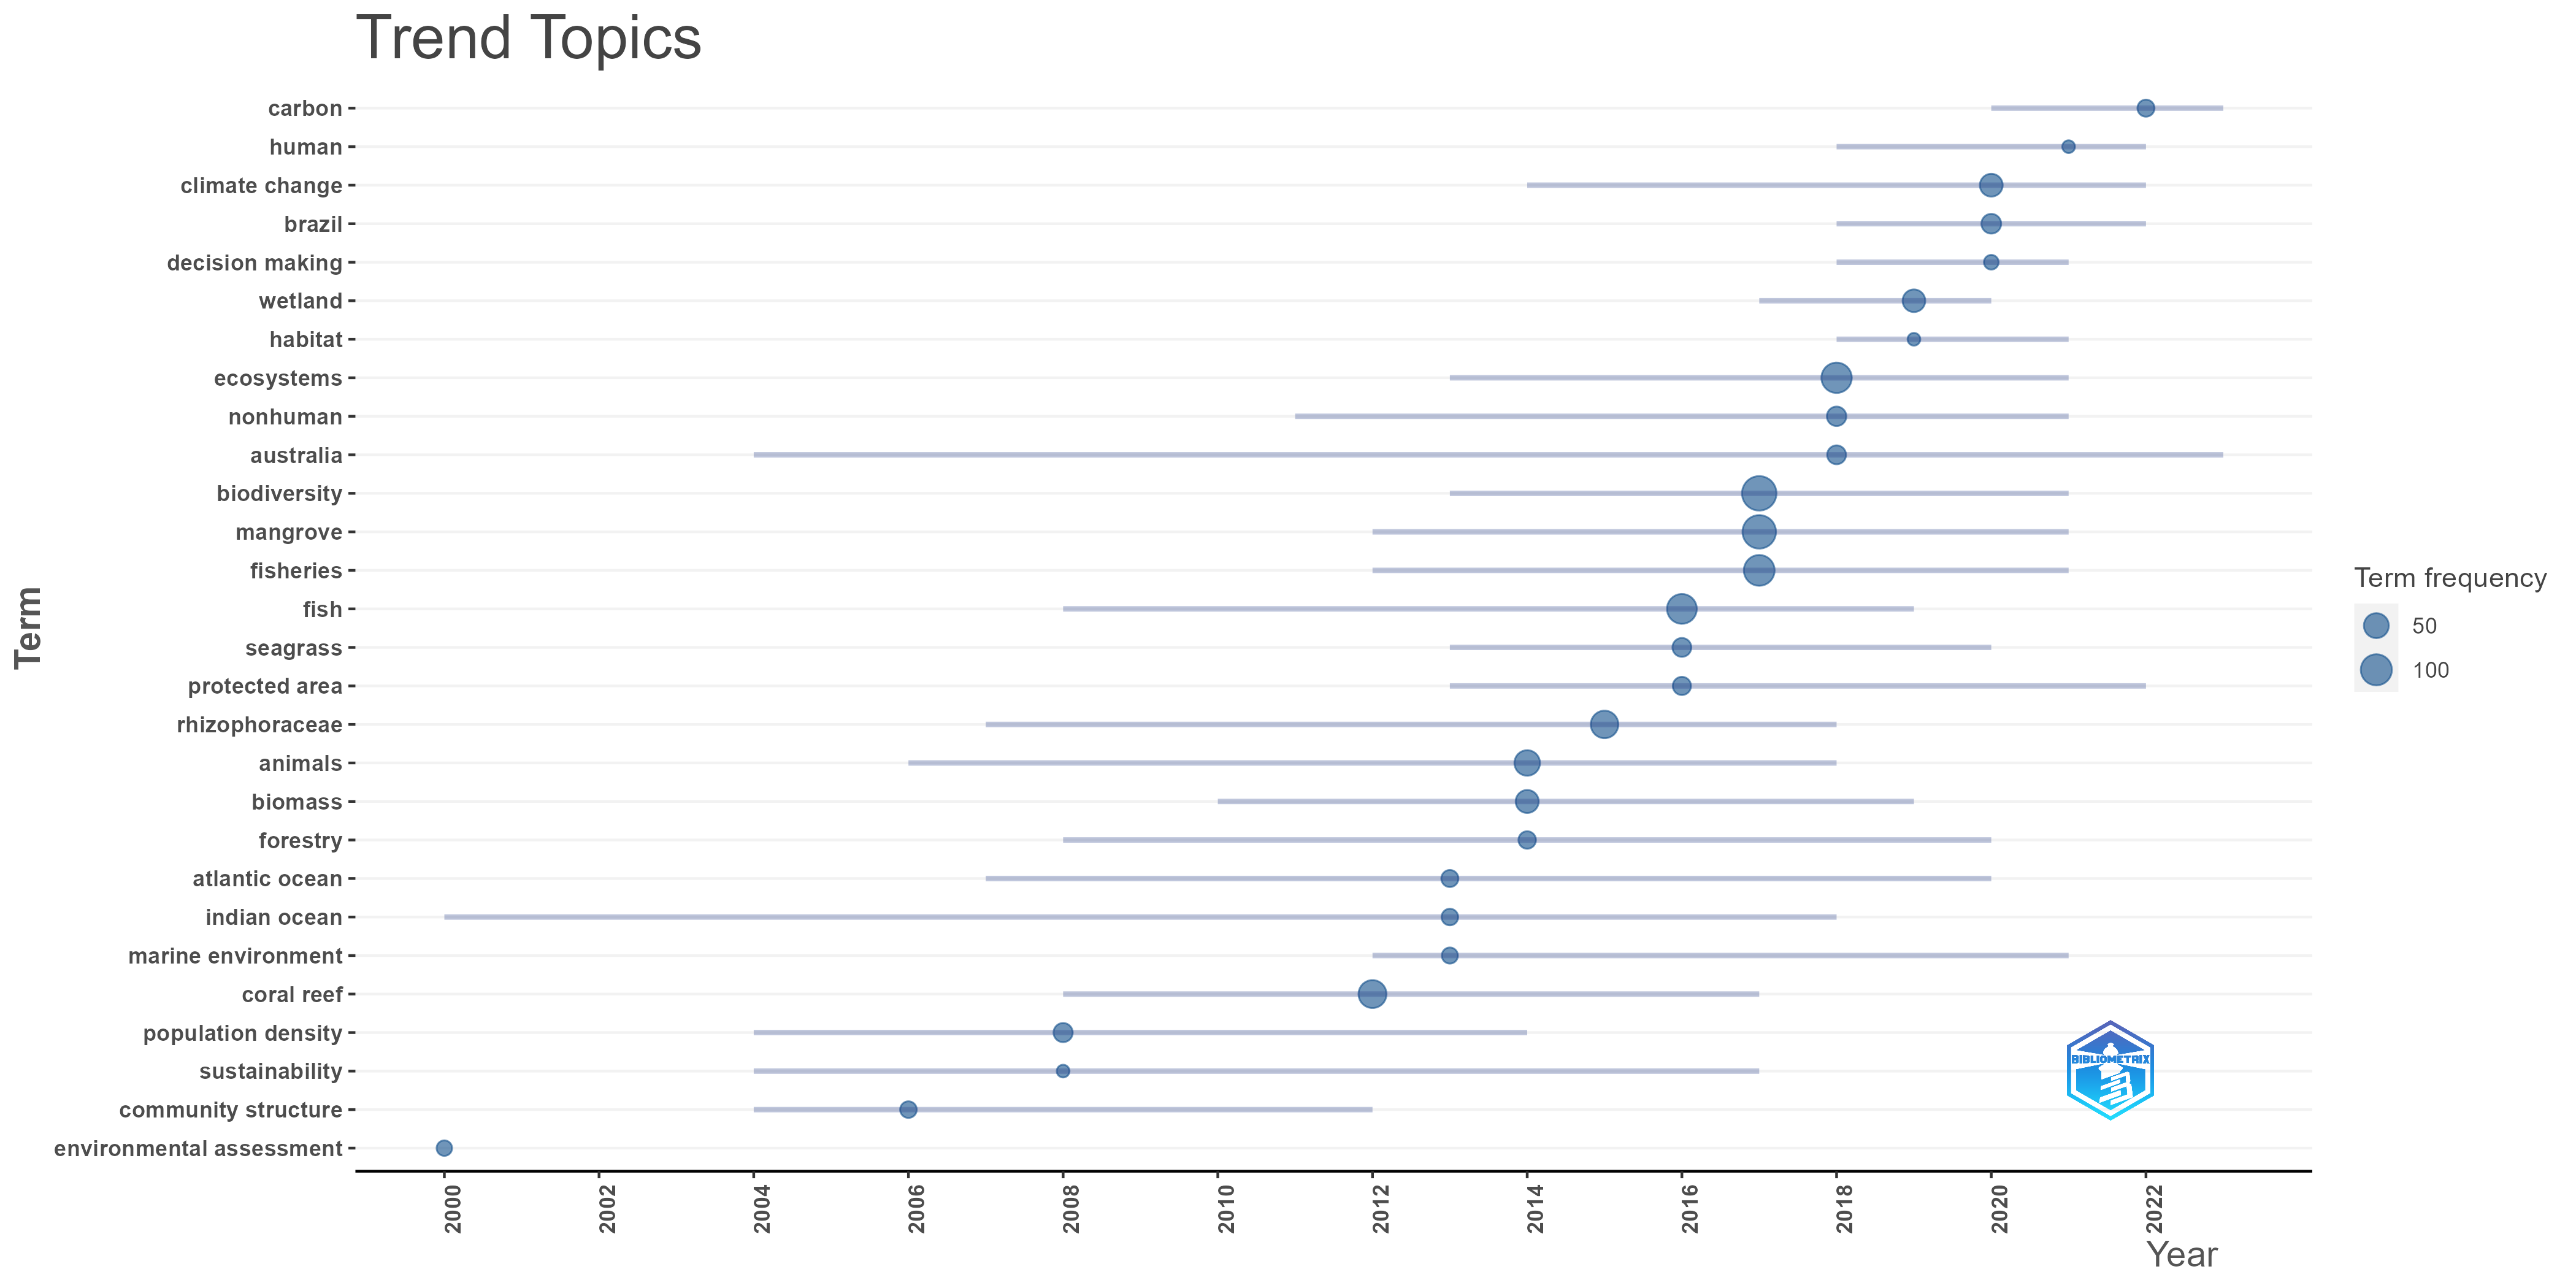
\includegraphics[width=1\linewidth]{TrendTopics} \caption{Fig Cap \label{TrendTopics}}\label{fig:TrendTopics}
\end{figure}



\begin{figure}
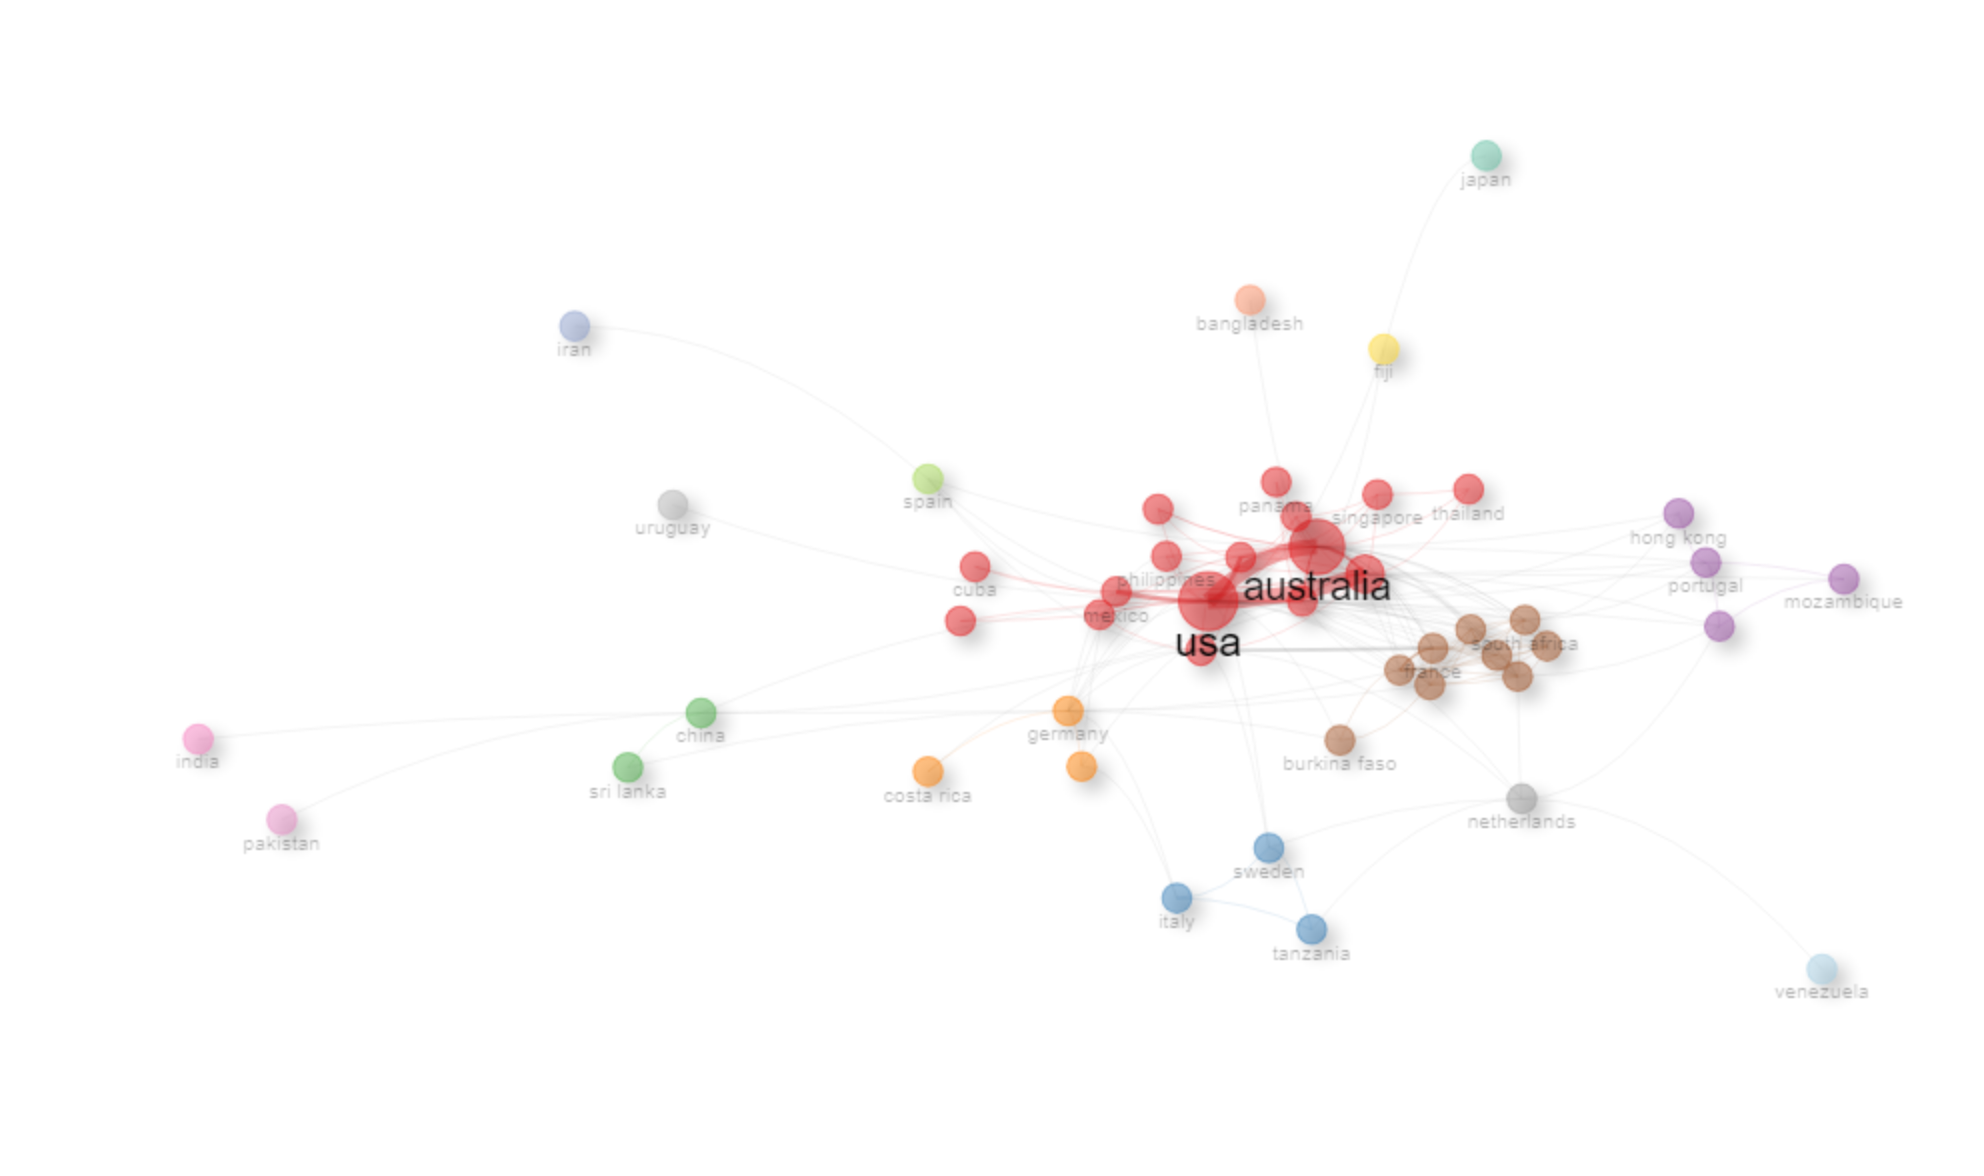
\includegraphics[width=1\linewidth]{CountryCollaborationNetwork} \caption{Fig Cap \label{CountryCollaborationNetwork}}\label{fig:CountryCollaborationNetwork}
\end{figure}



\hypertarget{refs}{}
\begin{CSLReferences}{1}{2}
\leavevmode\vadjust pre{\hypertarget{ref-aburto-oropezaMangrovesGulfCalifornia2008}{}}%
Aburto-Oropeza, O., Ezcurra, E., Danemann, G., Valdez, V., Murray, J., \& Sala, E. (2008). Mangroves in the {Gulf} of {California} increase fishery yields. \emph{Proceedings of the National Academy of Sciences}, \emph{105}(30), 10456--10459. \url{https://doi.org/10.1073/pnas.0804601105}

\leavevmode\vadjust pre{\hypertarget{ref-adeelAssessmentManagementMangrove2002}{}}%
Adeel, Z., \& Pomeroy, R. (2002). Assessment and management of mangrove ecosystems in developing countries. \emph{Trees}, \emph{16}(2-3), 235--238. \url{https://doi.org/10.1007/s00468-002-0168-4}

\leavevmode\vadjust pre{\hypertarget{ref-alongiMangroveForestsResilience2008}{}}%
Alongi, D. M. (2008). Mangrove forests: {Resilience}, protection from tsunamis, and responses to global climate change. \emph{Estuarine, Coastal and Shelf Science}, \emph{76}(1), 1--13. \url{https://doi.org/10.1016/j.ecss.2007.08.024}

\leavevmode\vadjust pre{\hypertarget{ref-alongiCarbonSequestrationMangrove2012}{}}%
Alongi, D. M. (2012). Carbon sequestration in mangrove forests. \emph{Carbon Management}, \emph{3}(3), 313--322. \url{https://doi.org/10.4155/cmt.12.20}

\leavevmode\vadjust pre{\hypertarget{ref-blueforestsAdaptiveCollaborativeManagement2012new}{}}%
Blue Forests. (2012). \emph{Adaptive {Collaborative} {Management} {Plan} for {Building} {Mangrove} {Resilience} in {Tanakeke} {Island}}.

\leavevmode\vadjust pre{\hypertarget{ref-cameronEstimatingFullGreenhouse2019}{}}%
Cameron, C., Hutley, L. B., \& Friess, D. A. (2019). Estimating the full greenhouse gas emissions offset potential and profile between rehabilitating and established mangroves. \emph{Science of The Total Environment}, \emph{665}, 419--431. \url{https://doi.org/10.1016/j.scitotenv.2019.02.104}

\leavevmode\vadjust pre{\hypertarget{ref-carugatiImpactMangroveForests2018}{}}%
Carugati, L., Gatto, B., Rastelli, E., Lo Martire, M., Coral, C., Greco, S., \& Danovaro, R. (2018). Impact of mangrove forests degradation on biodiversity and ecosystem functioning. \emph{Scientific Reports}, \emph{8}(1), 13298. \url{https://doi.org/10.1038/s41598-018-31683-0}

\leavevmode\vadjust pre{\hypertarget{ref-ellisonOriginsMangroveEcosystems1999}{}}%
Ellison, A. M., Farnsworth, E. J., \& Merkt, R. E. (1999). Origins of mangrove ecosystems and the mangrove biodiversity anomaly: {Mangrove} biodiversity anomaly. \emph{Global Ecology and Biogeography}, \emph{8}(2), 95--115. \url{https://doi.org/10.1046/j.1466-822X.1999.00126.x}

\leavevmode\vadjust pre{\hypertarget{ref-gilmanThreatsMangrovesClimate2008}{}}%
Gilman, E. L., Ellison, J., Duke, N. C., \& Field, C. (2008). Threats to mangroves from climate change and adaptation options: {A} review. \emph{Aquatic Botany}, \emph{89}(2), 237--250. \url{https://doi.org/10.1016/j.aquabot.2007.12.009}

\leavevmode\vadjust pre{\hypertarget{ref-nagelkerkenHabitatFunctionMangroves2008}{}}%
Nagelkerken, I., Blaber, S. J. M., Bouillon, S., Green, P., Haywood, M., Kirton, L. G., Meynecke, J.-O., Pawlik, J., Penrose, H. M., Sasekumar, A., \& Somerfield, P. J. (2008). The habitat function of mangroves for terrestrial and marine fauna: {A} review. \emph{Aquatic Botany}, \emph{89}(2), 155--185. \url{https://doi.org/10.1016/j.aquabot.2007.12.007}

\end{CSLReferences}

\end{document}
